% Options for packages loaded elsewhere
\PassOptionsToPackage{unicode}{hyperref}
\PassOptionsToPackage{hyphens}{url}
%
\documentclass[
]{article}
\usepackage{amsmath,amssymb}
\usepackage{lmodern}
\usepackage{iftex}
\ifPDFTeX
  \usepackage[T1]{fontenc}
  \usepackage[utf8]{inputenc}
  \usepackage{textcomp} % provide euro and other symbols
\else % if luatex or xetex
  \usepackage{unicode-math}
  \defaultfontfeatures{Scale=MatchLowercase}
  \defaultfontfeatures[\rmfamily]{Ligatures=TeX,Scale=1}
\fi
% Use upquote if available, for straight quotes in verbatim environments
\IfFileExists{upquote.sty}{\usepackage{upquote}}{}
\IfFileExists{microtype.sty}{% use microtype if available
  \usepackage[]{microtype}
  \UseMicrotypeSet[protrusion]{basicmath} % disable protrusion for tt fonts
}{}
\makeatletter
\@ifundefined{KOMAClassName}{% if non-KOMA class
  \IfFileExists{parskip.sty}{%
    \usepackage{parskip}
  }{% else
    \setlength{\parindent}{0pt}
    \setlength{\parskip}{6pt plus 2pt minus 1pt}}
}{% if KOMA class
  \KOMAoptions{parskip=half}}
\makeatother
\usepackage{xcolor}
\usepackage[margin=1in]{geometry}
\usepackage{color}
\usepackage{fancyvrb}
\newcommand{\VerbBar}{|}
\newcommand{\VERB}{\Verb[commandchars=\\\{\}]}
\DefineVerbatimEnvironment{Highlighting}{Verbatim}{commandchars=\\\{\}}
% Add ',fontsize=\small' for more characters per line
\usepackage{framed}
\definecolor{shadecolor}{RGB}{248,248,248}
\newenvironment{Shaded}{\begin{snugshade}}{\end{snugshade}}
\newcommand{\AlertTok}[1]{\textcolor[rgb]{0.94,0.16,0.16}{#1}}
\newcommand{\AnnotationTok}[1]{\textcolor[rgb]{0.56,0.35,0.01}{\textbf{\textit{#1}}}}
\newcommand{\AttributeTok}[1]{\textcolor[rgb]{0.77,0.63,0.00}{#1}}
\newcommand{\BaseNTok}[1]{\textcolor[rgb]{0.00,0.00,0.81}{#1}}
\newcommand{\BuiltInTok}[1]{#1}
\newcommand{\CharTok}[1]{\textcolor[rgb]{0.31,0.60,0.02}{#1}}
\newcommand{\CommentTok}[1]{\textcolor[rgb]{0.56,0.35,0.01}{\textit{#1}}}
\newcommand{\CommentVarTok}[1]{\textcolor[rgb]{0.56,0.35,0.01}{\textbf{\textit{#1}}}}
\newcommand{\ConstantTok}[1]{\textcolor[rgb]{0.00,0.00,0.00}{#1}}
\newcommand{\ControlFlowTok}[1]{\textcolor[rgb]{0.13,0.29,0.53}{\textbf{#1}}}
\newcommand{\DataTypeTok}[1]{\textcolor[rgb]{0.13,0.29,0.53}{#1}}
\newcommand{\DecValTok}[1]{\textcolor[rgb]{0.00,0.00,0.81}{#1}}
\newcommand{\DocumentationTok}[1]{\textcolor[rgb]{0.56,0.35,0.01}{\textbf{\textit{#1}}}}
\newcommand{\ErrorTok}[1]{\textcolor[rgb]{0.64,0.00,0.00}{\textbf{#1}}}
\newcommand{\ExtensionTok}[1]{#1}
\newcommand{\FloatTok}[1]{\textcolor[rgb]{0.00,0.00,0.81}{#1}}
\newcommand{\FunctionTok}[1]{\textcolor[rgb]{0.00,0.00,0.00}{#1}}
\newcommand{\ImportTok}[1]{#1}
\newcommand{\InformationTok}[1]{\textcolor[rgb]{0.56,0.35,0.01}{\textbf{\textit{#1}}}}
\newcommand{\KeywordTok}[1]{\textcolor[rgb]{0.13,0.29,0.53}{\textbf{#1}}}
\newcommand{\NormalTok}[1]{#1}
\newcommand{\OperatorTok}[1]{\textcolor[rgb]{0.81,0.36,0.00}{\textbf{#1}}}
\newcommand{\OtherTok}[1]{\textcolor[rgb]{0.56,0.35,0.01}{#1}}
\newcommand{\PreprocessorTok}[1]{\textcolor[rgb]{0.56,0.35,0.01}{\textit{#1}}}
\newcommand{\RegionMarkerTok}[1]{#1}
\newcommand{\SpecialCharTok}[1]{\textcolor[rgb]{0.00,0.00,0.00}{#1}}
\newcommand{\SpecialStringTok}[1]{\textcolor[rgb]{0.31,0.60,0.02}{#1}}
\newcommand{\StringTok}[1]{\textcolor[rgb]{0.31,0.60,0.02}{#1}}
\newcommand{\VariableTok}[1]{\textcolor[rgb]{0.00,0.00,0.00}{#1}}
\newcommand{\VerbatimStringTok}[1]{\textcolor[rgb]{0.31,0.60,0.02}{#1}}
\newcommand{\WarningTok}[1]{\textcolor[rgb]{0.56,0.35,0.01}{\textbf{\textit{#1}}}}
\usepackage{graphicx}
\makeatletter
\def\maxwidth{\ifdim\Gin@nat@width>\linewidth\linewidth\else\Gin@nat@width\fi}
\def\maxheight{\ifdim\Gin@nat@height>\textheight\textheight\else\Gin@nat@height\fi}
\makeatother
% Scale images if necessary, so that they will not overflow the page
% margins by default, and it is still possible to overwrite the defaults
% using explicit options in \includegraphics[width, height, ...]{}
\setkeys{Gin}{width=\maxwidth,height=\maxheight,keepaspectratio}
% Set default figure placement to htbp
\makeatletter
\def\fps@figure{htbp}
\makeatother
\setlength{\emergencystretch}{3em} % prevent overfull lines
\providecommand{\tightlist}{%
  \setlength{\itemsep}{0pt}\setlength{\parskip}{0pt}}
\setcounter{secnumdepth}{-\maxdimen} % remove section numbering
\ifLuaTeX
  \usepackage{selnolig}  % disable illegal ligatures
\fi
\IfFileExists{bookmark.sty}{\usepackage{bookmark}}{\usepackage{hyperref}}
\IfFileExists{xurl.sty}{\usepackage{xurl}}{} % add URL line breaks if available
\urlstyle{same} % disable monospaced font for URLs
\hypersetup{
  pdftitle={Projet Calcul Financier \& Statistique : En avant la musique !},
  pdfauthor={MAHI Riad \& Jérôme GAMBIEZ},
  hidelinks,
  pdfcreator={LaTeX via pandoc}}

\title{Projet Calcul Financier \& Statistique : En avant la musique !}
\author{MAHI Riad \& Jérôme GAMBIEZ}
\date{Mise à jour, le 25 Mai 2023}

\begin{document}
\maketitle

{
\setcounter{tocdepth}{2}
\tableofcontents
}
\hypertarget{introduction}{%
\subsection{1. Introduction}\label{introduction}}

Pour ce devoir de stastique nous avons choisi un sujet un peu original
qui est d'utiliser des musiques provenant de site de streaming connu
comme Spotify ou encore Youtube. Notre travail va être d'analyser un jeu
de donnée de 50 titres parmis les 5 artistes les plus connus des
plateforme afin d'en déduire une analyse sur des questions qu'on a pu se
poser notamment la corrélation entre genre en dancabilité. En effet,
plusieurs questions nous sont venu lors de la première étude du jeu de
donnée mais également en cours de route notammen, est-ce l'energie et la
dansabilité d'une musique ont une relation ? Est-ce l'énergie d'une
musique à un impact sur la sensibilité d'un utilisateur à aimer la
musique ? Même question pour la dansabilité? \newline

La source de notre jeu de donnée provient du site Kaggle.com: \newline
\url{https://www.kaggle.com/datasets/salvatorerastelli/spotify-and-youtube}

\textbf{Mise en place du jeu de donnée:}

\begin{Shaded}
\begin{Highlighting}[]
  \FunctionTok{library}\NormalTok{(ggplot2)}
  \FunctionTok{library}\NormalTok{(dplyr)}
\end{Highlighting}
\end{Shaded}

\begin{verbatim}
## 
## Attaching package: 'dplyr'
\end{verbatim}

\begin{verbatim}
## The following objects are masked from 'package:stats':
## 
##     filter, lag
\end{verbatim}

\begin{verbatim}
## The following objects are masked from 'package:base':
## 
##     intersect, setdiff, setequal, union
\end{verbatim}

\begin{Shaded}
\begin{Highlighting}[]
\NormalTok{  dataPath }\OtherTok{\textless{}{-}} \StringTok{"./Spotify\_Youtube.csv"}
\NormalTok{  data }\OtherTok{\textless{}{-}} \FunctionTok{read.csv}\NormalTok{(dataPath, }\AttributeTok{header=}\ConstantTok{TRUE}\NormalTok{, }\AttributeTok{stringsAsFactors=}\ConstantTok{FALSE}\NormalTok{, }\AttributeTok{nrows=}\DecValTok{50}\NormalTok{)}
\end{Highlighting}
\end{Shaded}

\textbf{Variables qualitative}\newline\newline Nous avons déduit à
partir des données extraites des variables qualitatives à minima
pertinente.

Notre première variable qualitative est de savoir si la musique est un
album ou un single, on la nomera \textbf{estAlbum}. Egalement, nous
avons choisi de prendre comme variable qualitative la \textbf{fréquence
d'écoute d'un titre}. Voici une définition des indicateurs de la
fréquence d'écoute en accord avec l'échelle des données que nous
possédons.

\begin{itemize}
\item
  Peu écouté : Cette catégorie désigne les chansons qui ont reçu un
  nombre de vues inférieur ou égal à 100 millions. Cela signifie que ces
  chansons ont été relativement moins populaires ou ont été moins
  diffusées en comparaison avec d'autres chansons.
\item
  Moyen écouté : Cette catégorie concerne les chansons qui ont reçu un
  nombre de vues compris entre 100 millions et 500 millions. Ces
  chansons peuvent être considérées comme ayant une popularité moyenne
  ou une diffusion modérée par rapport à d'autres chansons.
\item
  Très écouté : Cette catégorie comprend les chansons qui ont accumulé
  un nombre de vues supérieur à 500 millions. Ces chansons sont
  considérées comme ayant une grande popularité ou une diffusion élevée,
  attirant un grand nombre de spectateurs ou d'auditeurs.
\end{itemize}

\begin{Shaded}
\begin{Highlighting}[]
\CommentTok{\#Récupération de la colonne album\_type (album ou single)}
\NormalTok{album\_type }\OtherTok{\textless{}{-}} \FunctionTok{table}\NormalTok{(data}\SpecialCharTok{$}\NormalTok{Album\_type)}
\NormalTok{album\_type\_df }\OtherTok{\textless{}{-}} \FunctionTok{as.data.frame}\NormalTok{(album\_type)}
\NormalTok{album\_type\_df }\OtherTok{\textless{}{-}}\NormalTok{ album\_type\_df[}\FunctionTok{order}\NormalTok{(album\_type\_df}\SpecialCharTok{$}\NormalTok{Freq, }\AttributeTok{decreasing =} \ConstantTok{TRUE}\NormalTok{), ]}

\CommentTok{\#Récupération et traitement de la colonne fréquence écoute }
\NormalTok{data }\OtherTok{\textless{}{-}}\NormalTok{ data }\SpecialCharTok{\%\textgreater{}\%}
  \FunctionTok{mutate}\NormalTok{(}\AttributeTok{Freq\_listen =} \FunctionTok{case\_when}\NormalTok{(}
\NormalTok{    data}\SpecialCharTok{$}\NormalTok{Views }\SpecialCharTok{\textless{}=} \DecValTok{100000000} \SpecialCharTok{\textasciitilde{}} \StringTok{"peu écouté"}\NormalTok{,}
\NormalTok{    data}\SpecialCharTok{$}\NormalTok{Views }\SpecialCharTok{\textgreater{}} \DecValTok{100000000} \SpecialCharTok{\&}\NormalTok{ data}\SpecialCharTok{$}\NormalTok{Views }\SpecialCharTok{\textless{}=} \DecValTok{500000000} \SpecialCharTok{\textasciitilde{}} \StringTok{"moyen écouté"}\NormalTok{,}
\NormalTok{    data}\SpecialCharTok{$}\NormalTok{Views }\SpecialCharTok{\textgreater{}} \DecValTok{500000000} \SpecialCharTok{\textasciitilde{}} \StringTok{"très écouté"}\NormalTok{,}
    \ConstantTok{TRUE} \SpecialCharTok{\textasciitilde{}} \ConstantTok{NA\_character\_}
\NormalTok{  ))}

\NormalTok{freq\_listen }\OtherTok{\textless{}{-}} \FunctionTok{table}\NormalTok{(data}\SpecialCharTok{$}\NormalTok{Freq\_listen)}

\NormalTok{freq\_listen\_df }\OtherTok{\textless{}{-}} \FunctionTok{as.data.frame}\NormalTok{(freq\_listen)}
\NormalTok{freq\_listen\_df }\OtherTok{\textless{}{-}}\NormalTok{ freq\_listen\_df[}\FunctionTok{order}\NormalTok{(freq\_listen\_df}\SpecialCharTok{$}\NormalTok{Freq, }\AttributeTok{decreasing =} \ConstantTok{TRUE}\NormalTok{), ]}
\end{Highlighting}
\end{Shaded}

\textbf{Variables quantitative}\newline\newline Les variables
quantitatives sont \textbf{la dancabilité} d'une musique, qui est un
indicateur sur la probabilité de dancer sur une musique. Puis
\textbf{l'énergie} qui représente une mesure subjective qui nous aide à
évaluer et à caractériser le niveau d'intensité et d'activité ressenties
dans un morceau de musique.

\hypertarget{analyse-univariuxe9e}{%
\subsection{2. Analyse univariée}\label{analyse-univariuxe9e}}

\textbf{Répartitions des musiques album/single}

\begin{Shaded}
\begin{Highlighting}[]
\NormalTok{pie\_chart }\OtherTok{\textless{}{-}} \FunctionTok{ggplot}\NormalTok{(album\_type\_df, }\FunctionTok{aes}\NormalTok{(}\AttributeTok{x =} \StringTok{""}\NormalTok{, }\AttributeTok{y =}\NormalTok{ Freq, }\AttributeTok{fill =}\NormalTok{ Var1)) }\SpecialCharTok{+}
  \FunctionTok{geom\_bar}\NormalTok{(}\AttributeTok{stat =} \StringTok{"identity"}\NormalTok{, }\AttributeTok{width =} \DecValTok{1}\NormalTok{) }\SpecialCharTok{+}
  \FunctionTok{coord\_polar}\NormalTok{(}\StringTok{"y"}\NormalTok{, }\AttributeTok{start =} \DecValTok{0}\NormalTok{) }\SpecialCharTok{+}
  \FunctionTok{labs}\NormalTok{(}\AttributeTok{title =} \StringTok{"Répartition des types d\textquotesingle{}albums"}\NormalTok{, }\AttributeTok{fill =} \StringTok{"Type d\textquotesingle{}album"}\NormalTok{) }\SpecialCharTok{+}
  \FunctionTok{theme\_void}\NormalTok{() }\SpecialCharTok{+}
  \FunctionTok{geom\_text}\NormalTok{(}\FunctionTok{aes}\NormalTok{(}\AttributeTok{label =}\NormalTok{ Freq), }\AttributeTok{position =} \FunctionTok{position\_stack}\NormalTok{(}\AttributeTok{vjust =} \FloatTok{0.5}\NormalTok{), }\AttributeTok{size =} \DecValTok{4}\NormalTok{)}

\NormalTok{pie\_chart}
\end{Highlighting}
\end{Shaded}

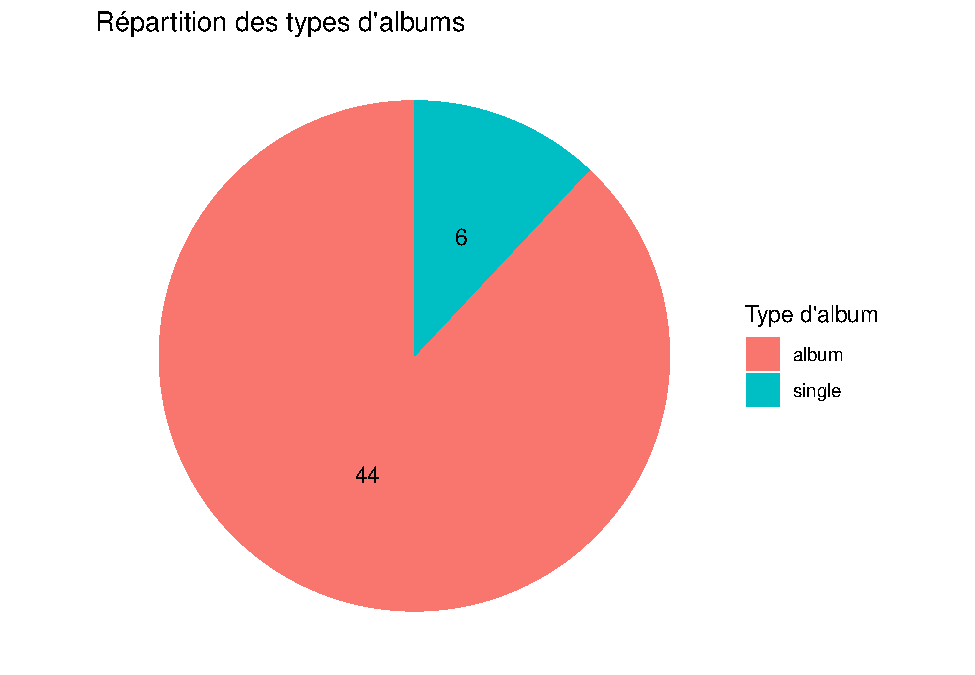
\includegraphics{spotify_analysis_files/figure-latex/unnamed-chunk-3-1.pdf}

On observe que parmis notre échantillon, il y a près de 90\% musique
provenant d'album et 10\% de single. Les titres d'albums sont dont
prédominant dans nos données.

\textbf{Répartition des fréquences d'écoute}

\begin{Shaded}
\begin{Highlighting}[]
\NormalTok{pie\_chart\_freq\_list }\OtherTok{\textless{}{-}} \FunctionTok{ggplot}\NormalTok{(freq\_listen\_df, }\FunctionTok{aes}\NormalTok{(}\AttributeTok{x =} \StringTok{""}\NormalTok{, }\AttributeTok{y =}\NormalTok{ Freq, }\AttributeTok{fill =}\NormalTok{ Var1)) }\SpecialCharTok{+}
  \FunctionTok{geom\_bar}\NormalTok{(}\AttributeTok{stat =} \StringTok{"identity"}\NormalTok{, }\AttributeTok{width =} \DecValTok{1}\NormalTok{) }\SpecialCharTok{+}
  \FunctionTok{coord\_polar}\NormalTok{(}\StringTok{"y"}\NormalTok{, }\AttributeTok{start =} \DecValTok{0}\NormalTok{) }\SpecialCharTok{+}
  \FunctionTok{labs}\NormalTok{(}\AttributeTok{title =} \StringTok{"Répartition par catégorie d\textquotesingle{}écoute"}\NormalTok{, }\AttributeTok{fill =} \StringTok{"Catégorie d\textquotesingle{}écoute"}\NormalTok{) }\SpecialCharTok{+}
  \FunctionTok{theme\_void}\NormalTok{() }\SpecialCharTok{+}
  \FunctionTok{geom\_text}\NormalTok{(}\FunctionTok{aes}\NormalTok{(}\AttributeTok{label =}\NormalTok{ Freq), }\AttributeTok{position =} \FunctionTok{position\_stack}\NormalTok{(}\AttributeTok{vjust =} \FloatTok{0.5}\NormalTok{), }\AttributeTok{size =} \DecValTok{4}\NormalTok{)}

\NormalTok{pie\_chart\_freq\_list}
\end{Highlighting}
\end{Shaded}

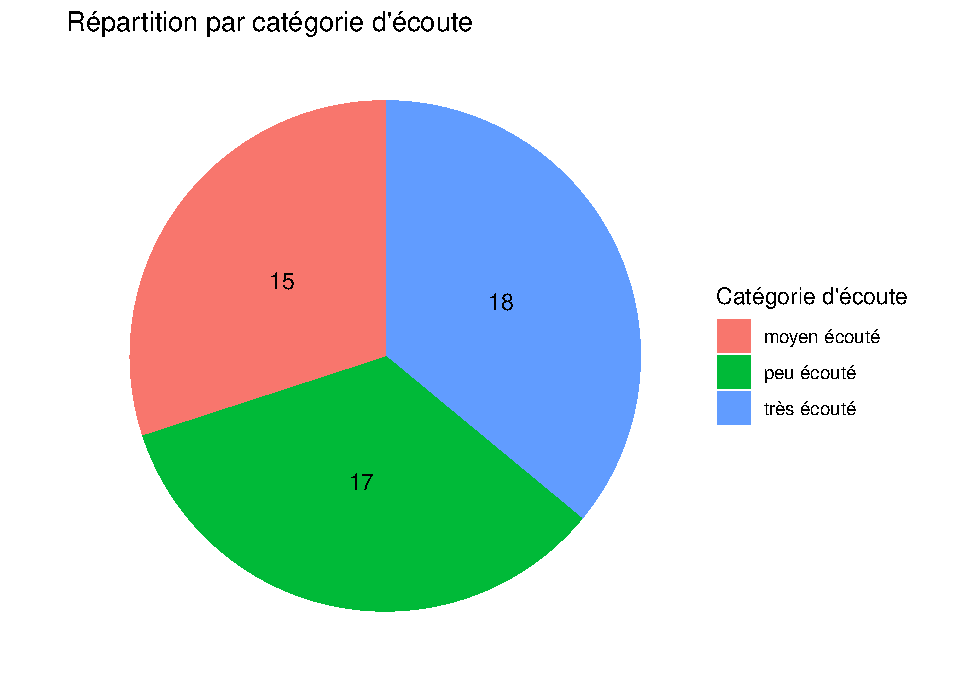
\includegraphics{spotify_analysis_files/figure-latex/unnamed-chunk-4-1.pdf}

On peut constater que nos fréquences d'écoutes sur les différents titres
de nos échantillons on la même proportion à un ou deux titres près.

\hypertarget{repruxe9sentation-graphique-de-la-ruxe9partition}{%
\subsubsection{Représentation graphique de la
répartition}\label{repruxe9sentation-graphique-de-la-ruxe9partition}}

\textbf{Dancabilité}

\begin{Shaded}
\begin{Highlighting}[]
\NormalTok{boxplot\_danceability }\OtherTok{\textless{}{-}} \FunctionTok{ggplot}\NormalTok{(data, }\FunctionTok{aes}\NormalTok{(}\AttributeTok{y =}\NormalTok{ Danceability)) }\SpecialCharTok{+}
  \FunctionTok{geom\_boxplot}\NormalTok{(}\AttributeTok{fill =} \StringTok{"lightblue"}\NormalTok{, }\AttributeTok{color =} \StringTok{"black"}\NormalTok{) }\SpecialCharTok{+}
  \FunctionTok{labs}\NormalTok{(}\AttributeTok{title =} \StringTok{"Distribution de la dançabilité"}\NormalTok{, }\AttributeTok{y =} \StringTok{"Dançabilité"}\NormalTok{) }\SpecialCharTok{+}
  \FunctionTok{theme\_minimal}\NormalTok{()}

\NormalTok{boxplot\_danceability}
\end{Highlighting}
\end{Shaded}

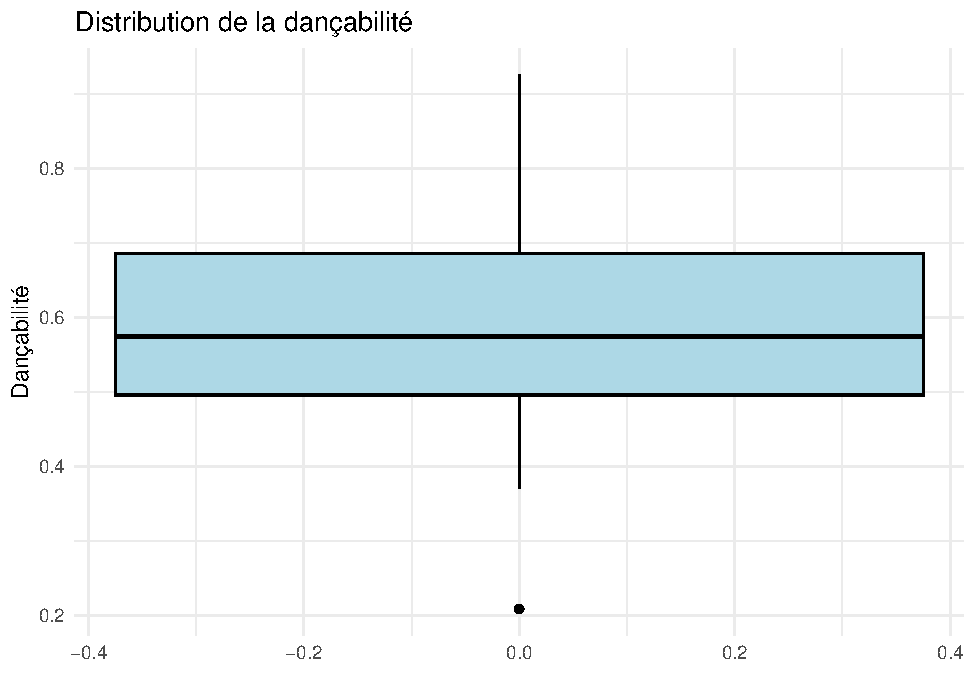
\includegraphics{spotify_analysis_files/figure-latex/unnamed-chunk-5-1.pdf}

En examinant le diagramme, on peut constater que la majorité des
musiques analysées, soit environ 58 \%, ont une danceability élevée.
Cela indique que ces morceaux sont adaptés à la danse et ont un
potentiel élevé pour inciter les gens à se déplacer et à bouger sur la
piste de danse.

De plus, le diagramme révèle que 25 \% des musiques ont un effet dansant
sur environ 70 \% de la population. Cela suggère que ces morceaux sont
particulièrement accrocheurs et entraînants, capables d'engager un large
public et de susciter l'envie de danser chez une majorité de personnes.

Enfin, il est intéressant de noter que 50 \% des musiques ont un effet
dansant sur une personne sur deux. Cela signifie que la danceability de
ces morceaux est plus subjective et peut varier d'une personne à
l'autre. Certains individus peuvent ressentir une forte envie de danser
en les écoutant, tandis que d'autres peuvent ne pas être aussi réceptifs
à leur effet dansant.

\textbf{Énergie}

\begin{Shaded}
\begin{Highlighting}[]
\NormalTok{boxplot\_energy }\OtherTok{\textless{}{-}} \FunctionTok{ggplot}\NormalTok{(data, }\FunctionTok{aes}\NormalTok{(}\AttributeTok{y =}\NormalTok{ Energy)) }\SpecialCharTok{+}
  \FunctionTok{geom\_boxplot}\NormalTok{(}\AttributeTok{fill =} \StringTok{"lightblue"}\NormalTok{, }\AttributeTok{color =} \StringTok{"black"}\NormalTok{) }\SpecialCharTok{+}
  \FunctionTok{labs}\NormalTok{(}\AttributeTok{title =} \StringTok{"Distribution de l\textquotesingle{}energie d\textquotesingle{}une musique"}\NormalTok{, }\AttributeTok{y =} \StringTok{"Énergie"}\NormalTok{) }\SpecialCharTok{+}
  \FunctionTok{theme\_minimal}\NormalTok{()}
\NormalTok{boxplot\_energy}
\end{Highlighting}
\end{Shaded}

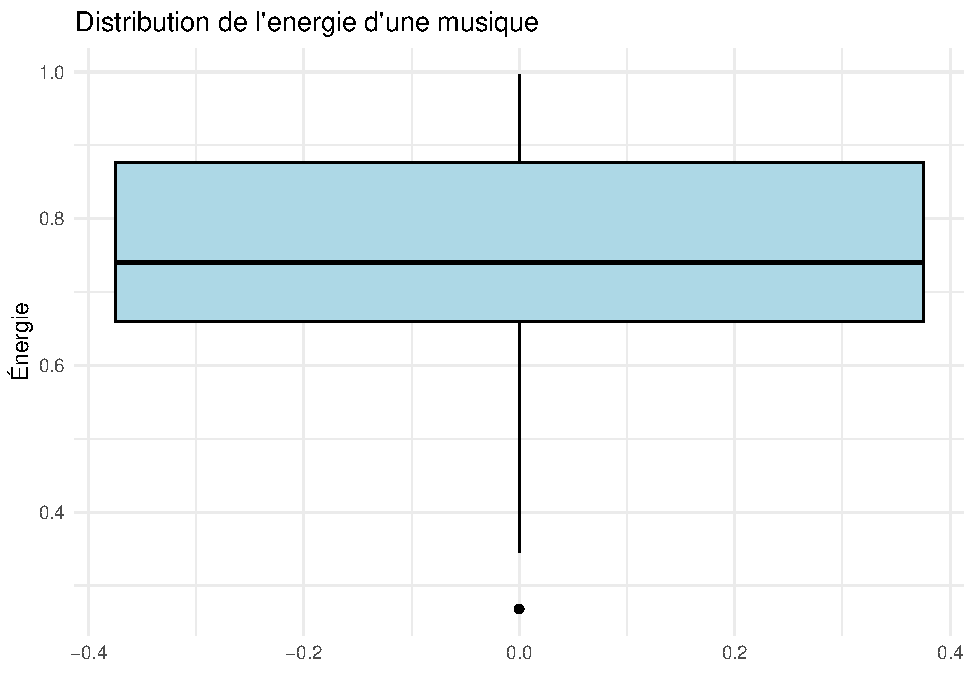
\includegraphics{spotify_analysis_files/figure-latex/unnamed-chunk-6-1.pdf}
L'analyse du diagramme en boîte à moustaches révèle plusieurs
informations importantes concernant l'énergie des morceaux de musique.
Plus l'énergie est proche de 1.0, plus elle est rapides, fortes et
bruyantes.

En examinant les différentes parties du diagramme, nous pouvons
constater que la médiane à 0.75. On peut donc conclure 75\% des morceaux
analysés présentent une énergie relativement élevée supérieur à 0.67.

La boîte à moustaches indique également que 25\% des morceaux ont une
énergie supérieure à 0,87, ce qui suggère une intensité, une vitesse et
un niveau sonore plus élevés. Ces morceaux pourraient correspondre à des
genres musicaux tels que le rock, le metal ou d'autres styles de musique
agressifs et dynamiques. On retrouve des groupes comme Metallica ou Red
Hot Chili Peppers.

D'autre part, 25\% des morceaux ont une énergie inférieure à 0,66, ce
qui indique une énergie plus basse. Ces morceaux pourraient être plus
calmes, plus lents et moins bruyants. On retrouve le musicien Coldlay
qui propose des musiques appelé Soft rock.

\textbf{Conclusion des deux moustaches}

En analysant les deux diagrammes ensemble, nous pouvons effectivement
observer une corrélation entre la danceability et l'énergie des morceaux
de musique. Il semble y avoir une tendance où les morceaux ayant une
forte danceability ont également une énergie élevée, supérieure à 0,65.

En se basant sur cette observation, il est intéressant de noter que les
musiques les plus dansantes sont celles de 50 Cent, un artiste de
hip-hop/rap. Ses morceaux ont une énergie se situant entre 0,65 et 0,75,
ce qui correspond à une intensité sonore élevée et une propension à
inciter les auditeurs à se déplacer et à danser. \#\# Estimation et
intervalles de confiance

\textbf{Analyse de la dancabilité}

\begin{Shaded}
\begin{Highlighting}[]
\NormalTok{dancabilite  }\OtherTok{\textless{}{-}}\NormalTok{ data}\SpecialCharTok{$}\NormalTok{Danceability}

\FunctionTok{var}\NormalTok{(dancabilite)}
\end{Highlighting}
\end{Shaded}

\begin{verbatim}
## [1] 0.0210791
\end{verbatim}

\begin{Shaded}
\begin{Highlighting}[]
\FunctionTok{mean}\NormalTok{(dancabilite)}
\end{Highlighting}
\end{Shaded}

\begin{verbatim}
## [1] 0.59372
\end{verbatim}

\begin{Shaded}
\begin{Highlighting}[]
\FunctionTok{par}\NormalTok{(}\AttributeTok{mfrow=}\FunctionTok{c}\NormalTok{(}\DecValTok{1}\NormalTok{,}\DecValTok{2}\NormalTok{))}
\FunctionTok{hist}\NormalTok{(dancabilite , }\AttributeTok{main=}\StringTok{"repartition de la dancabilité des musiques "}\NormalTok{,}\AttributeTok{xlab=}\StringTok{"dancabilite"}\NormalTok{,}\AttributeTok{prob=}\NormalTok{T)}
\FunctionTok{points}\NormalTok{(}\FunctionTok{seq}\NormalTok{(}\DecValTok{0}\NormalTok{,}\DecValTok{30}\NormalTok{,}\FloatTok{0.01}\NormalTok{),}\FunctionTok{dnorm}\NormalTok{(}\FunctionTok{seq}\NormalTok{(}\DecValTok{0}\NormalTok{,}\DecValTok{30}\NormalTok{,}\FloatTok{0.01}\NormalTok{),}\FunctionTok{mean}\NormalTok{(dancabilite),}\FunctionTok{sd}\NormalTok{(dancabilite)),}\AttributeTok{col=}\DecValTok{2}\NormalTok{,}\AttributeTok{type=}\StringTok{"l"}\NormalTok{)}
\FunctionTok{qqnorm}\NormalTok{(dancabilite)}
\FunctionTok{abline}\NormalTok{(}\FunctionTok{mean}\NormalTok{(dancabilite),}\FunctionTok{sd}\NormalTok{(dancabilite),}\AttributeTok{col=}\DecValTok{2}\NormalTok{)}
\end{Highlighting}
\end{Shaded}

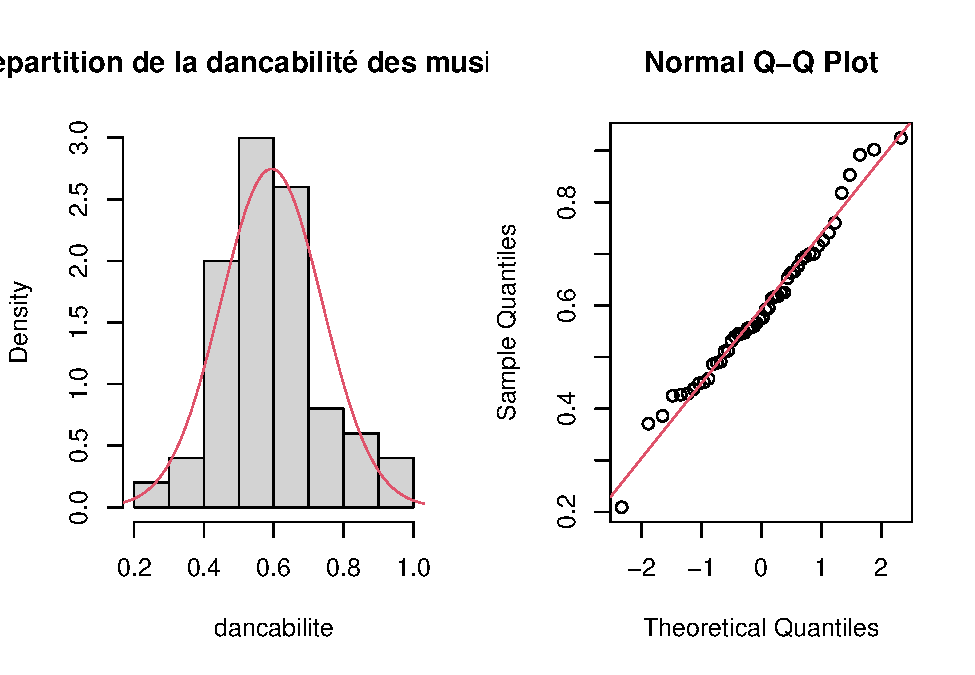
\includegraphics{spotify_analysis_files/figure-latex/unnamed-chunk-7-1.pdf}

\begin{Shaded}
\begin{Highlighting}[]
\NormalTok{interval}\OtherTok{=}\FunctionTok{t.test}\NormalTok{(dancabilite)}
\NormalTok{interval}\SpecialCharTok{$}\NormalTok{conf.int}
\end{Highlighting}
\end{Shaded}

\begin{verbatim}
## [1] 0.5524585 0.6349815
## attr(,"conf.level")
## [1] 0.95
\end{verbatim}

L'histogramme représente la répartition de la danceability des morceaux
de musique étudiés. La variable dancabilite a une variance (var) de
0.0210791 et une moyenne (mean) de 0.59372. Cela indique que les valeurs
de danceability sont relativement concentrées autour de la moyenne et
présentent une faible dispersion.

\textbf{Analyse de l'energie}

\begin{Shaded}
\begin{Highlighting}[]
\NormalTok{energie }\OtherTok{\textless{}{-}}\NormalTok{ data}\SpecialCharTok{$}\NormalTok{Energy}

\FunctionTok{var}\NormalTok{(energie)}
\end{Highlighting}
\end{Shaded}

\begin{verbatim}
## [1] 0.02873404
\end{verbatim}

\begin{Shaded}
\begin{Highlighting}[]
\FunctionTok{mean}\NormalTok{(energie)}
\end{Highlighting}
\end{Shaded}

\begin{verbatim}
## [1] 0.73938
\end{verbatim}

\begin{Shaded}
\begin{Highlighting}[]
\FunctionTok{par}\NormalTok{(}\AttributeTok{mfrow=}\FunctionTok{c}\NormalTok{(}\DecValTok{1}\NormalTok{,}\DecValTok{2}\NormalTok{))}
\FunctionTok{hist}\NormalTok{(energie , }\AttributeTok{main=}\StringTok{"repartition de l\textquotesingle{}energie des musiques "}\NormalTok{,}\AttributeTok{xlab=}\StringTok{"energie"}\NormalTok{,}\AttributeTok{prob=}\NormalTok{T)}
\FunctionTok{points}\NormalTok{(}\FunctionTok{seq}\NormalTok{(}\DecValTok{0}\NormalTok{,}\DecValTok{150}\NormalTok{,}\FloatTok{0.01}\NormalTok{),}\FunctionTok{dnorm}\NormalTok{(}\FunctionTok{seq}\NormalTok{(}\DecValTok{0}\NormalTok{,}\DecValTok{150}\NormalTok{,}\FloatTok{0.01}\NormalTok{),}\FunctionTok{mean}\NormalTok{(energie),}\FunctionTok{sd}\NormalTok{(energie)),}\AttributeTok{col=}\DecValTok{2}\NormalTok{,}\AttributeTok{type=}\StringTok{"l"}\NormalTok{)}
\FunctionTok{qqnorm}\NormalTok{(energie)}
\FunctionTok{abline}\NormalTok{(}\FunctionTok{mean}\NormalTok{(energie),}\FunctionTok{sd}\NormalTok{(energie),}\AttributeTok{col=}\DecValTok{2}\NormalTok{)}
\end{Highlighting}
\end{Shaded}

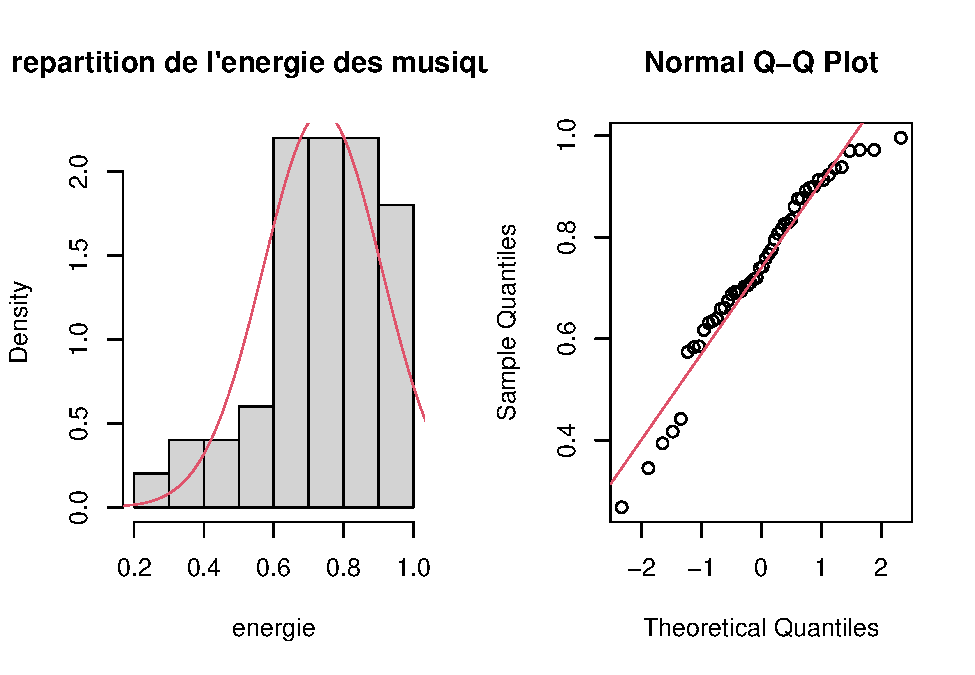
\includegraphics{spotify_analysis_files/figure-latex/unnamed-chunk-8-1.pdf}

\begin{Shaded}
\begin{Highlighting}[]
\NormalTok{interval}\OtherTok{=}\FunctionTok{t.test}\NormalTok{(energie)}
\NormalTok{interval}\SpecialCharTok{$}\NormalTok{conf.int}
\end{Highlighting}
\end{Shaded}

\begin{verbatim}
## [1] 0.6912055 0.7875545
## attr(,"conf.level")
## [1] 0.95
\end{verbatim}

\hypertarget{analyse-multivariuxe9e}{%
\subsection{3. Analyse multivariée}\label{analyse-multivariuxe9e}}

\hypertarget{analyse-quanti-x-quali}{%
\subsubsection{Analyse quanti x quali}\label{analyse-quanti-x-quali}}

Nous avons choisi de prendre comme varaible quantitative \textbf{la
dancabilité} et comme qualitative la \textbf{fréquence d'écoute d'un
titre}.

• Donner les résumés statistiques, histogrammes et/ou bloxplot par
sous-population.

\begin{Shaded}
\begin{Highlighting}[]
\FunctionTok{boxplot}\NormalTok{(data}\SpecialCharTok{$}\NormalTok{Danceability }\SpecialCharTok{\textasciitilde{}}\NormalTok{ data}\SpecialCharTok{$}\NormalTok{Freq\_listen, }\AttributeTok{main=}\StringTok{"Danceability en fonction de la fréquence d\textquotesingle{}écoute"}\NormalTok{, }\AttributeTok{xlab=}\StringTok{"Fréquence d\textquotesingle{}écoute"}\NormalTok{, }\AttributeTok{ylab=}\StringTok{"Danceability"}\NormalTok{)}
\end{Highlighting}
\end{Shaded}

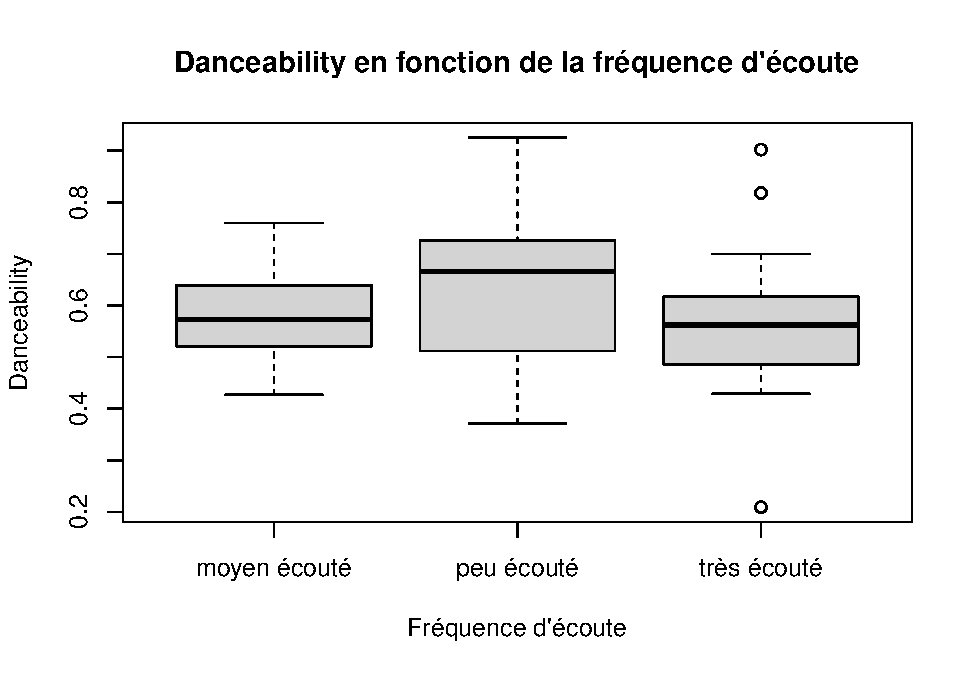
\includegraphics{spotify_analysis_files/figure-latex/unnamed-chunk-9-1.pdf}

On observe une répartition assez similaire entre les musiques
moyennement écoutées et les musiques très écoutées. Cependant, la
variable qui se démarque le plus est celle des musiques moyennement
écoutées, qui présente une danseabilité supérieure aux deux autres
variables. Toutefois, cette variable présente également une plus grande
dispersion que les deux autres. En effet, son premier quartile se situe
à une danseabilité de 0.3 et son troisième quartile à 0.9, avec une
médiane aux alentours de 0.7. En revanche, pour les deux autres
variables, le premier quartile se situe aux alentours de 0.45 et le
troisième quartile aux alentours de 0.7.

\begin{Shaded}
\begin{Highlighting}[]
\FunctionTok{summary}\NormalTok{(data}\SpecialCharTok{$}\NormalTok{Danceability[data}\SpecialCharTok{$}\NormalTok{Freq\_listen }\SpecialCharTok{==} \StringTok{"peu écouté"}\NormalTok{])}
\end{Highlighting}
\end{Shaded}

\begin{verbatim}
##    Min. 1st Qu.  Median    Mean 3rd Qu.    Max. 
##  0.3710  0.5120  0.6660  0.6312  0.7260  0.9250
\end{verbatim}

\begin{Shaded}
\begin{Highlighting}[]
\FunctionTok{summary}\NormalTok{(data}\SpecialCharTok{$}\NormalTok{Danceability[data}\SpecialCharTok{$}\NormalTok{Freq\_listen }\SpecialCharTok{==} \StringTok{"moyen écouté"}\NormalTok{])}
\end{Highlighting}
\end{Shaded}

\begin{verbatim}
##    Min. 1st Qu.  Median    Mean 3rd Qu.    Max. 
##  0.4270  0.5210  0.5730  0.5825  0.6390  0.7600
\end{verbatim}

\begin{Shaded}
\begin{Highlighting}[]
\FunctionTok{summary}\NormalTok{(data}\SpecialCharTok{$}\NormalTok{Danceability[data}\SpecialCharTok{$}\NormalTok{Freq\_listen }\SpecialCharTok{==} \StringTok{"très écouté"}\NormalTok{])}
\end{Highlighting}
\end{Shaded}

\begin{verbatim}
##    Min. 1st Qu.  Median    Mean 3rd Qu.    Max. 
##  0.2090  0.4873  0.5615  0.5677  0.6162  0.9020
\end{verbatim}

\textbf{Dancabilité par fréquence d'écoute:}

\begin{Shaded}
\begin{Highlighting}[]
\FunctionTok{par}\NormalTok{(}\AttributeTok{mfrow=}\FunctionTok{c}\NormalTok{(}\DecValTok{1}\NormalTok{,}\DecValTok{3}\NormalTok{))}
\FunctionTok{hist}\NormalTok{(data}\SpecialCharTok{$}\NormalTok{Danceability[data}\SpecialCharTok{$}\NormalTok{Freq\_listen }\SpecialCharTok{==} \StringTok{"peu écouté"}\NormalTok{], }\AttributeTok{main=}\StringTok{"peu écouté"}\NormalTok{, }\AttributeTok{xlab=}\StringTok{"Danceability"}\NormalTok{, }\AttributeTok{ylab=}\StringTok{"Fréquence"}\NormalTok{)}
\FunctionTok{hist}\NormalTok{(data}\SpecialCharTok{$}\NormalTok{Danceability[data}\SpecialCharTok{$}\NormalTok{Freq\_listen }\SpecialCharTok{==} \StringTok{"moyen écouté"}\NormalTok{], }\AttributeTok{main=}\StringTok{"moyen écouté"}\NormalTok{, }\AttributeTok{xlab=}\StringTok{"Danceability"}\NormalTok{, }\AttributeTok{ylab=}\StringTok{"Fréquence"}\NormalTok{)}
\FunctionTok{hist}\NormalTok{(data}\SpecialCharTok{$}\NormalTok{Danceability[data}\SpecialCharTok{$}\NormalTok{Freq\_listen }\SpecialCharTok{==} \StringTok{"très écouté"}\NormalTok{], }\AttributeTok{main=}\StringTok{"très écouté"}\NormalTok{, }\AttributeTok{xlab=}\StringTok{"Danceability"}\NormalTok{, }\AttributeTok{ylab=}\StringTok{"Fréquence"}\NormalTok{)}
\end{Highlighting}
\end{Shaded}

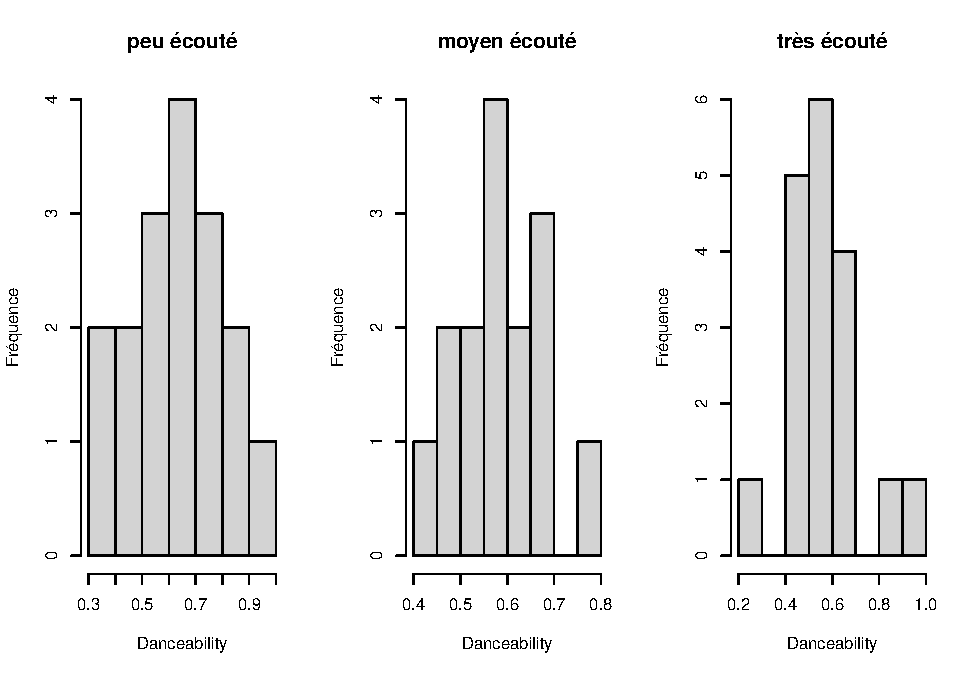
\includegraphics{spotify_analysis_files/figure-latex/unnamed-chunk-11-1.pdf}

\textbf{Calcule des rapports de corrélations:}

\begin{Shaded}
\begin{Highlighting}[]
\NormalTok{data}\SpecialCharTok{$}\NormalTok{Freq\_listen\_numeric }\OtherTok{\textless{}{-}} \FunctionTok{factor}\NormalTok{(data}\SpecialCharTok{$}\NormalTok{Freq\_listen)}
\NormalTok{data}\SpecialCharTok{$}\NormalTok{Freq\_listen\_numeric }\OtherTok{\textless{}{-}} \FunctionTok{as.numeric}\NormalTok{(data}\SpecialCharTok{$}\NormalTok{Freq\_listen\_numeric)}
\NormalTok{correlation }\OtherTok{\textless{}{-}} \FunctionTok{cor}\NormalTok{(dancabilite, data}\SpecialCharTok{$}\NormalTok{Freq\_listen\_numeric, }\AttributeTok{use =} \StringTok{"pairwise.complete.obs"}\NormalTok{)}
\NormalTok{correlation}
\end{Highlighting}
\end{Shaded}

\begin{verbatim}
## [1] -0.0513819
\end{verbatim}

Il existe une corrélation très faible et négative (-0.0513819) entre la
fréquence d'écoute et la danseabilité des musiques. Cela suggère qu'il
n'y a pas de relation significative entre ces deux variables dans
l'échantillon étudié. En d'autres termes, la fréquence d'écoute d'une
musique ne semble pas être un facteur déterminant de sa danseabilité, du
moins dans le contexte de ce jeu de données spécifique.

Cela signifie que, d'après les données analysées, il n'existe qu'une
très légère tendance indiquant que plus un morceau de musique est écouté
fréquemment, moins il est susceptible d'être dansant. Cependant, il est
important de noter que cette corrélation est proche de zéro, ce qui
suggère qu'il n'y a pas de relation linéaire significative entre la
danseabilité et la fréquence d'écoute des morceaux.

Ce résultat suggère qu'il y a pas de preuve pour dire qu'une fréquence
d'écoute élevée soit directement liée à une danseabilité.

• Faire le test d'égalité des moyennes. Spécifier les hypothèses.
Conclure ?

Hypothèses :

Hypothèse nulle (H0) : Il n'y a pas de différence significative entre
les moyennes des groupes de fréquence d'écoute.

Hypothèse alternative (H1) : Il existe une différence significative
entre au moins deux des moyennes des groupes de fréquence d'écoute.

\begin{Shaded}
\begin{Highlighting}[]
\CommentTok{\# Effectuer le test d\textquotesingle{}ANOVA}
\NormalTok{model }\OtherTok{\textless{}{-}} \FunctionTok{aov}\NormalTok{(Danceability }\SpecialCharTok{\textasciitilde{}}\NormalTok{ Freq\_listen, }\AttributeTok{data =}\NormalTok{ data)}

\CommentTok{\# Résumé des résultats}
\FunctionTok{summary}\NormalTok{(model)}
\end{Highlighting}
\end{Shaded}

\begin{verbatim}
##             Df Sum Sq Mean Sq F value Pr(>F)
## Freq_listen  2 0.0379 0.01896   0.896  0.415
## Residuals   47 0.9950 0.02117
\end{verbatim}

Nous avons utilisé un seuil de signification de 0,05 pour évaluer la
différence entre les groupes. La valeur p calculée pour notre test est
de 0,723, ce qui est supérieur à notre seuil de signification. Cela
signifie que nous n'avons pas trouvé suffisamment de preuves
statistiques pour rejeter l'hypothèse nulle.

Nos résultats indiquent qu'il n'y a pas de différence significative dans
la danseabilité des morceaux de musique en fonction de la fréquence
d'écoute. Autrement dit, que les morceaux soient peu écoutés,
moyennement écoutés ou très écoutés, cela n'a pas d'impact
statistiquement significatif sur leur danseabilité.

\hypertarget{analyse-quali-x-quali}{%
\subsubsection{Analyse quali x quali}\label{analyse-quali-x-quali}}

Nous avons choisi de prendre comme varaible qualitative
\textbf{estAlbum} et la \textbf{fréquence d'écoute d'un titre}.
Maintenant, nous allons procéder au test d'indépendance pour évaluer
s'il existe une relation significative entre ces deux variables.

• Faire le tableau de contingence, proposer une représentation
graphique.

Lors de l'analyse de notre jeu de données, nous avons constaté que la
répartition entre les singles et les albums était déséquilibrée, avec
seulement 6 singles (12\%) et 44 albums (88\%) :

\begin{Shaded}
\begin{Highlighting}[]
\FunctionTok{table}\NormalTok{(data}\SpecialCharTok{$}\NormalTok{Album\_type)}
\end{Highlighting}
\end{Shaded}

\begin{verbatim}
## 
##  album single 
##     44      6
\end{verbatim}

Cette répartition peut avoir une incidence sur nos conclusions, car les
données ne sont pas homogènes. Il faut noter que la taille de
l'échantillon de singles est relativement petite, ce qui peut affecter
la représentativité de nos résultats.

\begin{Shaded}
\begin{Highlighting}[]
\CommentTok{\# Tableau de contingence}
\NormalTok{table\_contingency }\OtherTok{\textless{}{-}} \FunctionTok{table}\NormalTok{(data}\SpecialCharTok{$}\NormalTok{Freq\_listen, data}\SpecialCharTok{$}\NormalTok{Album\_type)}

\CommentTok{\# Affichage du tableau de contingence}
\FunctionTok{print}\NormalTok{(table\_contingency)}
\end{Highlighting}
\end{Shaded}

\begin{verbatim}
##               
##                album single
##   moyen écouté    15      0
##   peu écouté      11      6
##   très écouté     18      0
\end{verbatim}

\begin{Shaded}
\begin{Highlighting}[]
\CommentTok{\# Graphique}
\NormalTok{contingency }\OtherTok{\textless{}{-}} \FunctionTok{barplot}\NormalTok{(table\_contingency, }\AttributeTok{main=}\StringTok{"Fréquence d\textquotesingle{}écoute en fonction du type d\textquotesingle{}album"}\NormalTok{, }
        \AttributeTok{xlab=}\StringTok{"Fréquence d\textquotesingle{}écoute"}\NormalTok{, }\AttributeTok{ylab=}\StringTok{"Nombre de morceaux"}\NormalTok{, }\AttributeTok{col=}\FunctionTok{c}\NormalTok{(}\StringTok{"blue"}\NormalTok{, }\StringTok{"red"}\NormalTok{, }\StringTok{"orange"}\NormalTok{),}
        \AttributeTok{legend =} \FunctionTok{c}\NormalTok{(}\StringTok{"Peu écouté"}\NormalTok{, }\StringTok{"Moyen écouté"}\NormalTok{, }\StringTok{"Très écouté"}\NormalTok{))}
\end{Highlighting}
\end{Shaded}

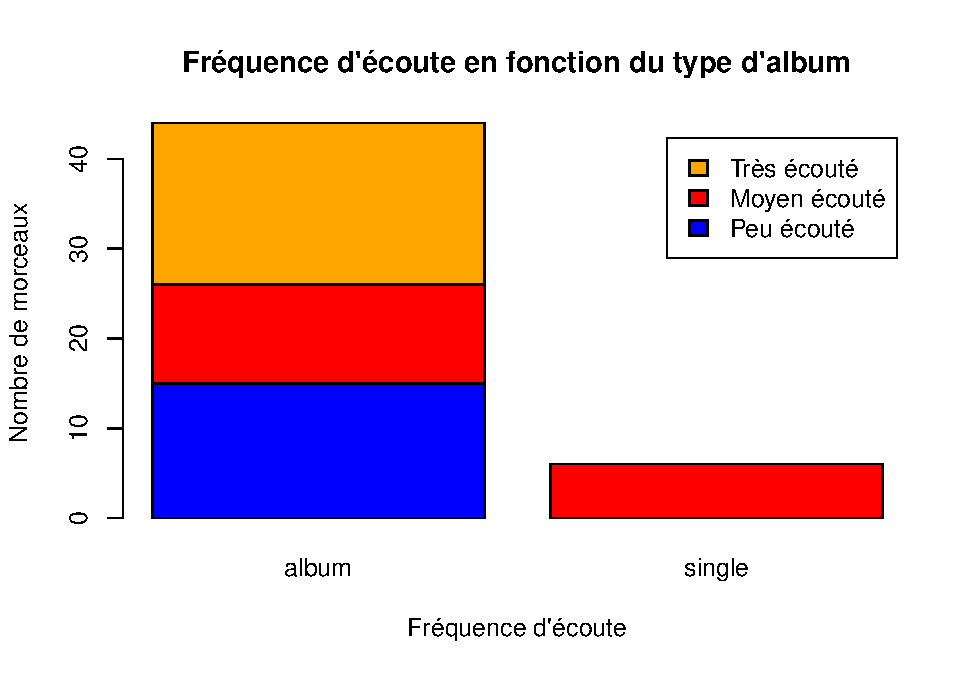
\includegraphics{spotify_analysis_files/figure-latex/unnamed-chunk-15-1.pdf}

\begin{Shaded}
\begin{Highlighting}[]
\NormalTok{contingency}
\end{Highlighting}
\end{Shaded}

\begin{verbatim}
## [1] 0.7 1.9
\end{verbatim}

Nous observons que la fréquence d'écoute des morceaux de musique ne
semble pas être influencée par le fait qu'ils soient inclus dans un
album ou qu'ils soient des singles. Cela indique que la présence d'un
morceau dans un album ne garantit pas nécessairement qu'il sera plus
écouté ou moins écouté.

Malgré que tous les singles soit dans la catégorie ``Moyen écouté cela
ne veut pas dire qu'un sigle sera forcement dans cette catégorie.

En conclusion, les résultats actuels ne permettent pas de tirer des
conclusions solides sur la relation entre le type d'album (album ou
single) et la fréquence d'écoute des morceaux de musique.

• Faire le test d'indépendance. Spécifier les hypothèses. Conclure ?

Pour effectuer le test d'indépendance, nous formulons les hypothèses
suivantes :

Hypothèse nulle (H0) : La fréquence d'écoute d'un titre est indépendante
du type d'album. Hypothèse alternative (H1) : La fréquence d'écoute d'un
titre est dépendante du type d'album. Pour effectuer le test, nous
utiliserons une analyse de chi-carré (test du chi-carré d'indépendance).
Ce test nous permettra de déterminer si les différences observées entre
les fréquences d'écoute et le type d'album sont statistiquement
significatives.

Je vais maintenant procéder à l'exécution du test d'indépendance.
Veuillez patienter un instant.

\begin{Shaded}
\begin{Highlighting}[]
\NormalTok{table\_contingency }\OtherTok{\textless{}{-}} \FunctionTok{table}\NormalTok{(data}\SpecialCharTok{$}\NormalTok{Freq\_listen, data}\SpecialCharTok{$}\NormalTok{Album\_type)}

\CommentTok{\# Test d\textquotesingle{}indépendance (chi{-}carré)}
\NormalTok{result }\OtherTok{\textless{}{-}} \FunctionTok{chisq.test}\NormalTok{(table\_contingency)}
\end{Highlighting}
\end{Shaded}

\begin{verbatim}
## Warning in chisq.test(table_contingency): Chi-squared approximation may be
## incorrect
\end{verbatim}

\begin{Shaded}
\begin{Highlighting}[]
\FunctionTok{print}\NormalTok{(result)}
\end{Highlighting}
\end{Shaded}

\begin{verbatim}
## 
##  Pearson's Chi-squared test
## 
## data:  table_contingency
## X-squared = 13.235, df = 2, p-value = 0.001337
\end{verbatim}

Sur la base de ces résultats, nous pouvons conclure ce qui suit :

La valeur de p obtenue (0.001337) est inférieure à notre seuil de
significativité de 0.05. Par conséquent, nous rejetons l'hypothèse nulle
selon laquelle la fréquence d'écoute d'un titre est indépendante du type
d'album.

Cela suggère qu'il existe une relation significative entre la fréquence
d'écoute des morceaux de musique et le type d'album (album ou single).
En d'autres termes, le type d'album a une influence sur la fréquence
d'écoute des morceaux.

\hypertarget{analyse-quanti-x-quanti}{%
\subsubsection{Analyse quanti x quanti}\label{analyse-quanti-x-quanti}}

Noys avons choisi de prendre comme varaible quantitative \textbf{la
dancabilité} et l'\textbf{energie}.

• Tracer le nuage de point, tracer la droite des moindre carrés

\begin{Shaded}
\begin{Highlighting}[]
  \CommentTok{\# Nuage de points}
  \FunctionTok{plot}\NormalTok{(data}\SpecialCharTok{$}\NormalTok{Danceability, data}\SpecialCharTok{$}\NormalTok{Energy, }\AttributeTok{main=}\StringTok{"Danceability en fonction de l\textquotesingle{}Energy"}\NormalTok{, }
      \AttributeTok{xlab=}\StringTok{"Danceability"}\NormalTok{, }\AttributeTok{ylab=}\StringTok{"Energy"}\NormalTok{, }\AttributeTok{pch=}\DecValTok{19}\NormalTok{)}

  \CommentTok{\# Droite des moindres carrés}
  \FunctionTok{abline}\NormalTok{(}\FunctionTok{lm}\NormalTok{(data}\SpecialCharTok{$}\NormalTok{Energy }\SpecialCharTok{\textasciitilde{}}\NormalTok{ data}\SpecialCharTok{$}\NormalTok{Danceability), }\AttributeTok{col=}\StringTok{"red"}\NormalTok{)}
\end{Highlighting}
\end{Shaded}

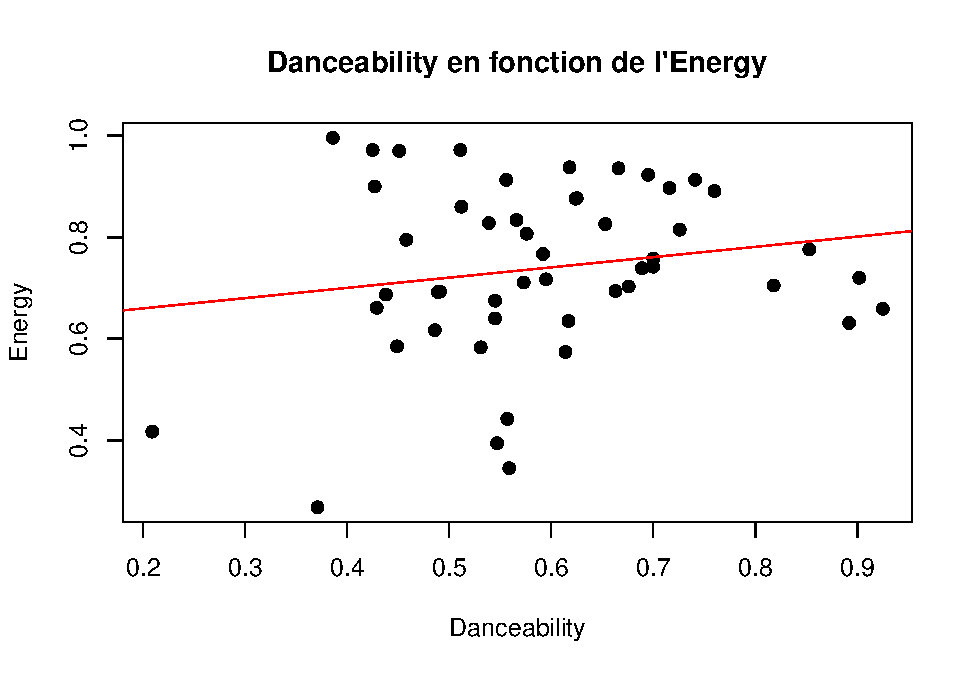
\includegraphics{spotify_analysis_files/figure-latex/unnamed-chunk-17-1.pdf}

• Calculer le coefficient de corrélation linéaire

\begin{Shaded}
\begin{Highlighting}[]
\CommentTok{\# Calcul du coefficient de corrélation linéaire}
\FunctionTok{cor}\NormalTok{(data}\SpecialCharTok{$}\NormalTok{Danceability, data}\SpecialCharTok{$}\NormalTok{Energy)}
\end{Highlighting}
\end{Shaded}

\begin{verbatim}
## [1] 0.1730491
\end{verbatim}

Après avoir calculé le coefficient de corrélation linéaire entre les
variables ``Danceability'' et ``Energy'', nous obtenons un résultat de
0.1730491.

Ce coefficient de corrélation linéaire mesure la force et la direction
de la relation linéaire entre les deux variables. Dans notre cas, le
coefficient de corrélation est proche de zéro, ce qui suggère une faible
corrélation linéaire entre la dancabilité et l'énergie des morceaux de
musique.

• Tester la pertinence de la régression linéaire. Conclure

\begin{Shaded}
\begin{Highlighting}[]
\CommentTok{\# Régression linéaire}
\NormalTok{model }\OtherTok{\textless{}{-}} \FunctionTok{lm}\NormalTok{(data}\SpecialCharTok{$}\NormalTok{Energy }\SpecialCharTok{\textasciitilde{}}\NormalTok{ data}\SpecialCharTok{$}\NormalTok{Danceability)}

\CommentTok{\# Résumé des résultats}
\FunctionTok{summary}\NormalTok{(model)}
\end{Highlighting}
\end{Shaded}

\begin{verbatim}
## 
## Call:
## lm(formula = data$Energy ~ data$Danceability)
## 
## Residuals:
##      Min       1Q   Median       3Q      Max 
## -0.42638 -0.08757 -0.01924  0.13110  0.29859 
## 
## Coefficients:
##                   Estimate Std. Error t value Pr(>|t|)    
## (Intercept)         0.6194     0.1014   6.109 1.71e-07 ***
## data$Danceability   0.2020     0.1660   1.217    0.229    
## ---
## Signif. codes:  0 '***' 0.001 '**' 0.01 '*' 0.05 '.' 0.1 ' ' 1
## 
## Residual standard error: 0.1687 on 48 degrees of freedom
## Multiple R-squared:  0.02995,    Adjusted R-squared:  0.009737 
## F-statistic: 1.482 on 1 and 48 DF,  p-value: 0.2294
\end{verbatim}

Après avoir effectué la régression linéaire de la variable ``Energy'' en
fonction de la variable ``Danceability'' L'équation de régression
obtenue est : Energy = 0.6194 + 0.2020 * Danceability. Cela signifie que
pour chaque unité d'augmentation de la dancabilité, on peut s'attendre à
une augmentation de 0.2020 dans l'énergie des morceaux de musique.

L'estimation du coefficient d'interception est de 0.6194 avec une erreur
standard de 0.1014. Ce coefficient représente la valeur de l'énergie
lorsque la dancabilité est égale à zéro. De même pour l'estimation du
coefficient de pente de la dancabilité est de 0.2020 avec une erreur
standard de 0.1660.

Le test de significativité pour la pente dancabilité montre un t-value
de 1.217 et une valeur de p de 0.229. Cette valeur de p élevée indique
que la relation entre la dancabilité et l'énergie n'est pas
significative dans notre modèle.

L'analyse de variance (F-statistic) donne une valeur de 1.482 avec un
degré de liberté de 1 et 48. Le p-value associé est de 0.2294, ce qui
indique que le modèle de régression dans son ensemble n'est pas
significatif.

Pour conclure, les résultats obtenu dans notre analyse de régression
linéaire, il n'y a pas suffisamment de preuves pour soutenir la
pertinence du modèle de régression linéaire pour prédire l'énergie des
morceaux de musique en fonction de leur dancabilité. La dancabilité
seule ne semble pas être un prédicteur significatif de l'énergie.
D'autres facteurs ou variables pourraient être nécessaires pour
améliorer la pertinence du modèle.

\end{document}
